\chapter{Central Dogma of Molecular Biology}

The {\em central dogma of molecular biology} is a key idea that explains how genetic information is used in living organisms. Proposed by Francis Crick in 1958, it describes the flow of information from DNA to RNA, and then to proteins, which perform most of the vital functions in cells. This concept has been foundational to the field of molecular biology and continues to shape our understanding of genetics.

\begin{marginfigure}
    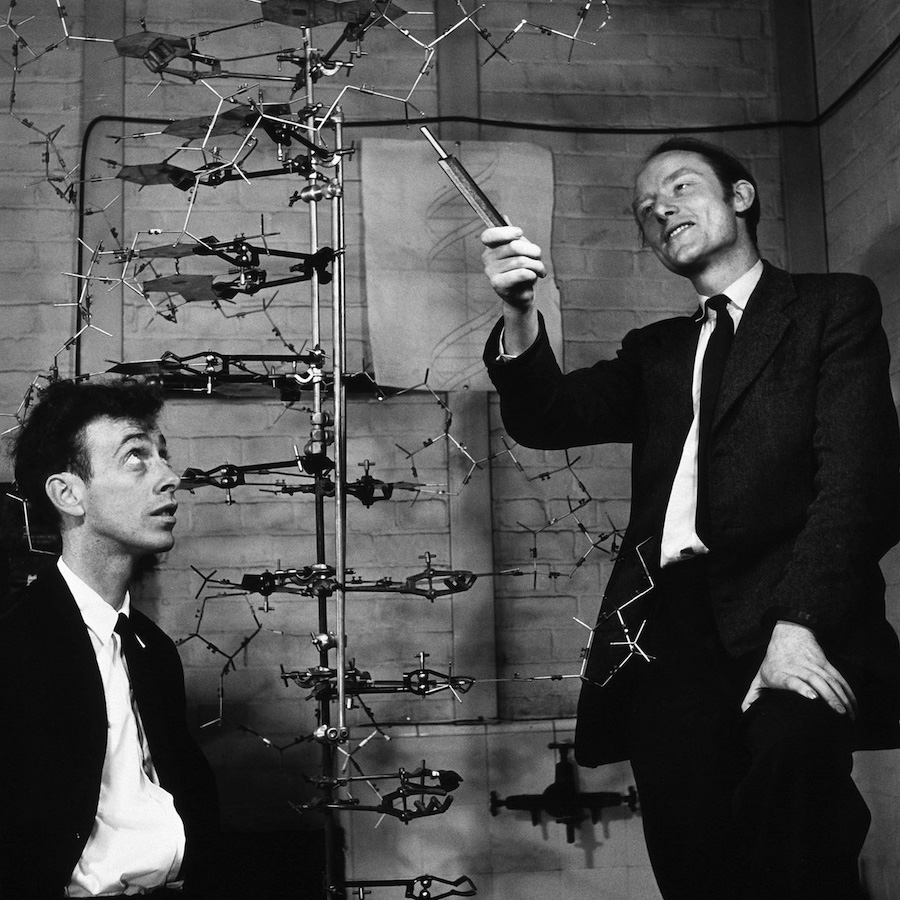
\includegraphics{figs/history/watson-crick-dna.jpeg}
    \caption[6pt]{Francis Crick and James Watson with their famous model of DNA.}
    \label{fig:watson-crick-dna}
\end{marginfigure}

Here are som of the major milestones, and some of accompanying stories, in the development of the central dogma of molecular biology:

\medskip\noindent\textbf{1953:} The double-helix structure of DNA was uncovered by James Watson, Francis Crick, and Rosalind Franklin. Franklin’s X-ray diffraction work was crucial in understanding the structure of DNA, although her contribution was underappreciated at the time. Without her clear images, the puzzle of DNA’s structure might have remained unsolved for much longer.

\begin{marginfigure}
    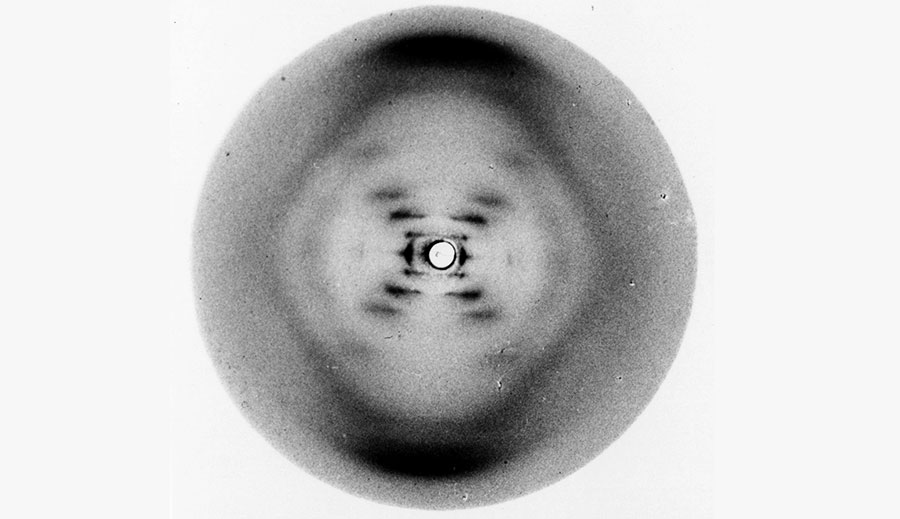
\includegraphics{figs/history/photograph-51.jpeg}
    \caption[6pt]{Photograph 51, the X-ray diffraction image of DNA taken by Rosalind Franklin.}
    \label{fig:photograph-51}
\end{marginfigure}

James Watson and Francis Crick's famous paper, titled "Molecular Structure of Nucleic Acids: A Structure for Deoxyribose Nucleic Acid," was published on April 25, 1953 in the journal Nature. This landmark paper was only about one page long but had a profound impact on biology, as it described the double-helix structure of DNA for the first time.

Towards the end of Watson and Crick’s 1953 paper, there is a famous sentence that reads:
\begin{quote}
    \textit{It has not escaped our notice that the specific pairing we have postulated immediately suggests a possible copying mechanism for the genetic material.}
\end{quote}
This sentence is understated yet profound. In a single line, Watson and Crick hint at one of the most important implications of their discovery: the double-helix structure of DNA naturally explains how genetic information can be copied during cell division. The specific pairing between the nucleotide bases (adenine with thymine, and guanine with cytosine) suggested a mechanism by which each strand of the DNA molecule could serve as a template for creating a new, complementary strand. This was a subtle but powerful insight, as it laid the foundation for understanding DNA replication—a central process in biology that ensures genetic continuity from one generation to the next. The modest tone of the sentence belied its transformative impact on genetics and molecular biology.

Notice that the discovery of the structure of DNA was hard and not without faults, even by the most influential scientists of the time. Linus Pauling, one of the most renowned chemists of the era, proposed a triple-helix model for DNA in 1953, placing the phosphate backbone in the center and the nucleotide bases on the outside. This model was fundamentally flawed due to charge repulsion between phosphate groups and its failure to account for base pairing. Pauling’s proposal, though influential, did not align with emerging experimental data, which ultimately led to the correct double-helix structure by Watson and Crick.

\begin{marginfigure}
    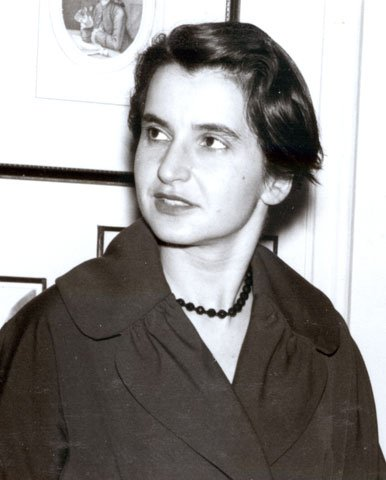
\includegraphics{figs/history/rosalind-franklin.jpeg}
    \caption[6pt]{Rosalind Franklin.}
    \label{fig:franklin}
\end{marginfigure}

\medskip\noindent\textbf{1958:} Francis Crick introduced the central dogma, explaining that information flows in one direction: from DNA to RNA to proteins. Proteins are the molecules that perform most functions within a cell, and they are produced according to instructions stored in DNA.

\medskip\noindent\textbf{1961:} François Jacob and Jacques Monod discovered messenger RNA (mRNA), which showed that RNA carries instructions from DNA to the cell's protein factories. This helped confirm that RNA acts as a temporary messenger in the process of turning genetic information into proteins.

\medskip\noindent\textbf{1966:} The cracking of the genetic code was a major scientific breakthrough. A group of scientists, including \textit{Marshall Nirenberg}, \textit{Har Gobind Khorana}, and members of the \textit{RNA Tie Club}, worked tirelessly to decipher how sequences of RNA are translated into amino acids, which are the building blocks of proteins. The \textit{RNA Tie Club} was an informal but competitive group of 20 scientists, each member representing one of the 20 amino acids. They wore black silk ties emblazoned with the symbol for RNA. Despite the serious goal of cracking the genetic code, there was a sense of humor and camaraderie in the group.

An anecdote is that they created their own membership pins and made grand declarations, like ``each amino acid will be solved by a club member!'' However, the race to crack the code was so competitive that, in the end, the discoveries were made by a few scientists outside the club. Still, the members’ friendly competition and idea-sharing helped push the field forward.

\bigskip\noindent\textbf{1970:} Howard Temin and David Baltimore discovered reverse transcriptase, an enzyme that allows RNA to be copied back into DNA. This discovery overturned the assumption that the flow of genetic information was strictly one-way and provided crucial insights into how retroviruses like HIV function.

\bigskip\noindent
For computer scientists, the central dogma provides a blueprint for how biological data is organized. DNA is the database, RNA acts as a dynamic intermediary, and proteins are the functional outcomes. In bioinformatics, understanding these relationships is key to analyzing genetic sequences, predicting protein structures, and exploring the effects of mutations.